\chapter{Schwingungsvorgänge}
schwingfähiges System \\
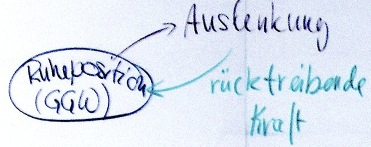
\includegraphics{Bild211}

\section{Energiebetrachtung}
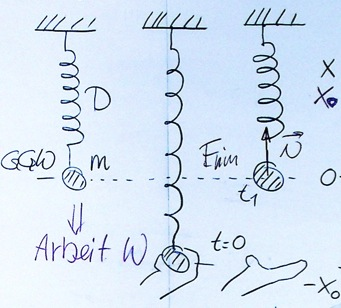
\includegraphics{Bild212} \\
\begin{itemize}
	\item gegeben durch Schwingsystem
	\item Anfangsbedingungen
\end{itemize}
harmonische Schwingung
\[ x(t) = \underbrace{x_0}_{\text{Amplitude}} \sin( \underbrace{\omega_0}_{\text{Kreisfrequenz}} t + \underbrace{\phi_0}_{\text{Phase}} ) \]
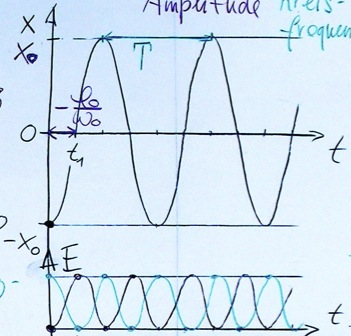
\includegraphics{Bild213}
\[
	E_{\text{tot}} = E_{\text{pot}} + E_{\text{kin}} = \text{ konst. } = W \\
	E_{\text{pot}} = \frac{1}{2} D x^2 \\
	E_{\text{kin}} = \frac{1}{2} m \dot{x}^2
\]
Kreisfrequenz $\omega_0$
\[ \text{(2.N.P.)} \quad \omega_o = \sqrt{\frac{D}{m}} \]
Schwingungsperiode $T$
\[ \boxed{ T = \frac{2\pi}{\omega_0} } \]
Frequenz $f = \frac{1}{T} = \frac{\omega_0}{2\pi}$

\begin{rep*}
	\uline{Das Induktionsgesetz} \\
	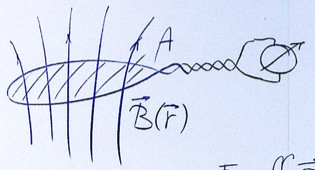
\includegraphics{Bild214} \\
	magn. Fluss
	\[ \Phi = \iint \vec{B} \cdot \vec{\dd A} \]
	Faraday's Induktionsgesetz
	\[ \boxed{ U_{\text{ind}} = -\frac{\dd \Phi}{\dd t} } \]
	
	\uline{Schwingungsvorgänge} \\
	\uline{harmonische Schwingung:}
	\[ \boxed{ x(t) = \underbrace*{x_0}_{\text{Amplitude}} \sin( \underbrace{\omega_0}_{\text{Kreisfrequenz}} t + \underbrace{\phi_0}_{\text{Phase}} ) } \]
	\begin{bsp*}[ note = Federpendel ]
		\[ \omega_0 = \sqrt{\frac{D}{m}} \]
	\end{bsp*}
	\uline{Energieerhaltung}\\
	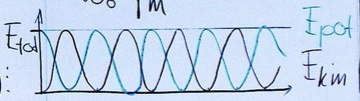
\includegraphics{Bild215}
	\[ E_{\text{tot}} = E_{\text{kin}}(t) + E_{\text{pot}}(t) = \frac{1}{2} m \dot{x}^2(t) + \frac{1}{2} D x^2(t) = W = \text{ konst.} \]
\end{rep*}

\section{Gedämpfte Schwingung}
Energie geht durch Reibung verloren! \\
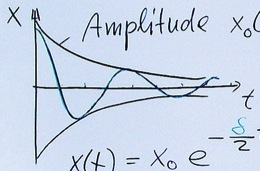
\includegraphics{Bild216}
\[
	\text{Amplitude } x_0(t) = x e^{-\frac{\delta}{2} t} \\
	x(t) = x_0 e^{-\frac{\delta}{2} t} \sin( \omega_d t + \phi_0 )
\]
schwache Dämpfung ($\delta$ klein) $\omega_d \approx \omega_0$
Energieverlust: $E_{\text{tot}} = E_{\text{pot}}( 0 ) \cdot e^{-\delta t}$

\section{Erzwungene Schwingung}
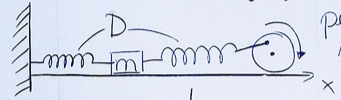
\includegraphics{Bild217} \\
periodische Anregung $F_0 \sin \omega t$ \\
2 Frequenzen!
\begin{itemize}
	\item ohne Anregung: $\omega_0 = \sqrt{\frac{D}{m}}$ Eigenfrequenz
	\item Anregungsfrequenz $\omega$ frei wählbar
\end{itemize}
Frage: Bewegung mit $\omega$ oder $\omega_0$? \\
Zu Beginn: Einschwingung mit $\omega_0$ (gedämpft) und $\omega$! \\
$t \rightarrow$ gross: stationärer Zustand. Nur noch $\omega$!

\subsection{Nur noch stationärer Zustand}
(mit Dämpfung: rasch im stationärem Zustand)
\[ \boxed{ x(t) = x_0(\omega) \cdot \sin( \omega t + \phi(\omega) ) } \]
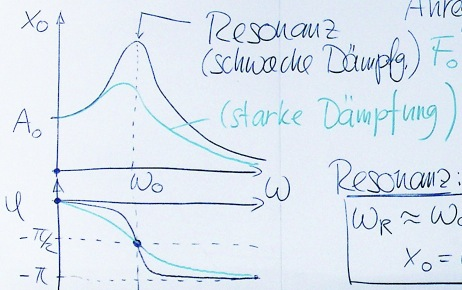
\includegraphics{Bild218} \\
Anregung: $F_0 \sin \omega t$ \\
Resonanz:
\[ \boxed{ \omega_R \approx \omega_0 , \phi = -\frac{\pi}{2} , x_0 = \text{ maximal} } \]

\subsection{Erklärung der Phase bei Resonanz}
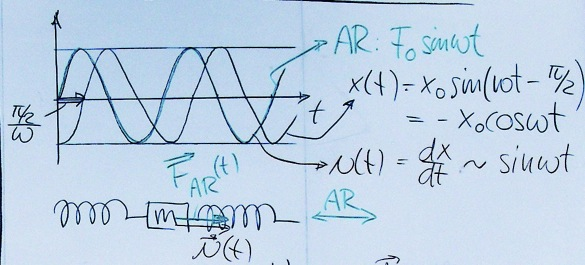
\includegraphics{Bild219}
\[ x(t) = x_0 \sin( \omega t - \frac{\pi}{2} = - x_0 \cos \omega t \]
$\implies$ Verschiebung $\vec{\dd r}$ \\
$\implies \vec{F_{AR}}$ verrichtet immer positive Arbeit!

\section{Anwendung: Magnetische Resonanztomographie (MRI)}
\subsection{Wasserstoffkern}
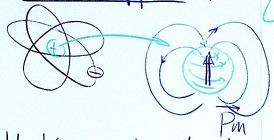
\includegraphics{Bild220} \\
\begin{itemize}
	\item Ladung $+e$
	\item Eigendrehimplus (Spin)
	\item magn. Moment $\vec{p_m}$
\end{itemize}
\subsection{\texorpdfstring{\ce{H}}{H}-Kerne in starkem Magnetfeld}
$\drsh$ magn. Moment $\vec{p_m}$ + Drehimpuls \\
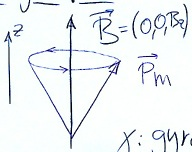
\includegraphics{Bild221} \\
$\implies$ Präzessionsbewegung \\
\[
	\vec{B} = ( 0 , 0 , B_z )
	\intertext{Präzessions-(Larmor-)Frequenz}
	\boxed{ \omega_L = \gamma \cdot B_z }
\]
$\gamma$: gyromagn. Verhältnis \\
Wasserstoffkern: $\gamma = 2\pi \cdot \SI{42.58}{\mega\hertz\per\tesla}$

\subsection{Kernresonanz-Spektroskopie}
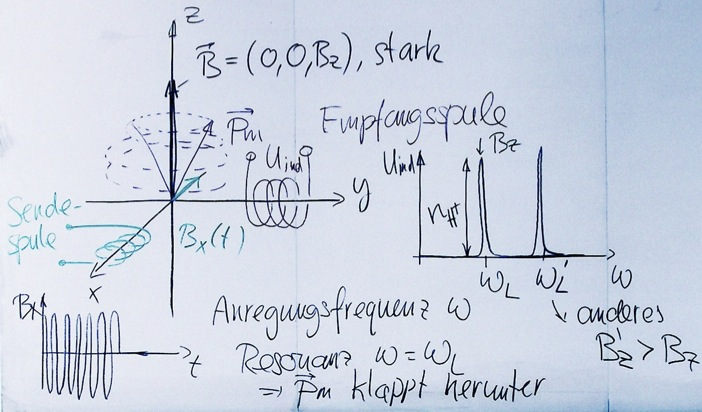
\includegraphics{Bild222} \\
Anregungsfrequenz $\omega$ \\
Resonanz $\omega = \omega_L$ \\
$\implies \vec{p_m}$ klappt herunter

















